%% PRE EDITION
\documentclass[a4paper]{article}
\usepackage[utf8]{inputenc}
\usepackage[T1]{fontenc}
\usepackage[french]{babel}
\usepackage{soul}
\usepackage[pdftex]{graphicx}

\usepackage{amsfonts}
\usepackage{amsthm}
\usepackage{amsmath}
\usepackage{amssymb}
\usepackage{mathrsfs}
\usepackage{booktabs}
\usepackage{siunitx}
\usepackage{thmtools}

%% LAYOUT
\declaretheoremstyle[
    bodyfont=\normalfont\color{red},
    headfont=\color{red}
]{styleattention}

\declaretheoremstyle[
    spacebelow=1em
]{styleremarque}

\declaretheoremstyle[
    spaceabove=-6pt, 
    spacebelow=6pt, 
    headfont=\normalfont\bfseries, 
    bodyfont = \normalfont,
    postheadspace=1em, 
    qed=$\Box$, 
    headpunct={$\rhd$}
]{mystyle} 

\declaretheorem[thmbox=M,numberwithin=section,title=Définition]{definition}
\declaretheorem[thmbox=M,sibling=definition]{proposition}
\declaretheorem[thmbox=M,sibling=definition]{corollaire}
\declaretheorem[thmbox=M,sibling=definition,title=Théorème]{theoreme}
\declaretheorem[thmbox=M,sibling=definition]{lemme}
\declaretheorem[thmbox=M,sibling=definition,title=Propriété]{propriete}
\declaretheorem[thmbox=M,sibling=definition,title=Propriétés]{proprietes}
\declaretheorem[style=styleremarque,sibling=definition,title=Remarque]{remarque}
\declaretheorem[style=styleattention,title=À revoir]{Arevoir}
\declaretheorem[name={}, style=mystyle, unnumbered]{preuve}


\renewcommand\qedsymbol{$\blacksquare$}

%% NEW COMMAND
\newcommand{\mass}{\mathrm{M}}
\newcommand{\pol}{a}
\newcommand{\dep}{b}

\usepackage{geometry}
\geometry{hmargin=3cm,vmargin=2.5cm}

\usepackage{tabularx}
\usepackage{float}

\title{Premier résultat sur la polymérisation}
\author{Cécile Della Valle}

%% DEBUT DE REDACTION
\begin{document}

\maketitle

%%%%%%%%%%%%%%%%%%%%%%%%%%%%%%%%%%%%%%%%%%%%%%%%%%%%%%%%%%%%%%%%%%%%%%%%%%%%%%%%%%%%%%%%%%%%%%%%%%%%%%%%%%%%%%%%%%%%%%%%%%%%%%%%%
%%%%%%%%%%%%%%%%%%%%%%%%%%%%%%%%%%%%%%%%%%%%%%%%%%%%%%%%%%%%%%%%%%%%%%%%%%%%%%%%%%%%%%%%%%%%%%%%%%%%%%%%%%%%%%%%%%%%%%%%%%%%%%%%%
%%%%%%%%%%%%%%%%%%%%%%%%%%%%%%%%%%%%%%%%%%%%%%%%%%%%%%%%%%%%%%%%%%%%%%%%%%%%%%%%%%%%%%%%%%%%%%%%%%%%%%%%%%%%%%%%%%%%%%%%%%%%%%%%%
\section{Introduction}
%%%%%%%%%%%%%%%%%%%%%%%%%%%%%%%%%%%%%%%%%%%%%%%%%%%%%%%%%%%%%%%%%%%%%%%%%%%%%%%%%%%%%%%%%%%%%%%%%%%%%%%%%%%%%%%%%%%%%%%%%%%%%%%%%
%%%%%%%%%%%%%%%%%%%%%%%%%%%%%%%%%%%%%%%%%%%%%%%%%%%%%%%%%%%%%%%%%%%%%%%%%%%%%%%%%%%%%%%%%%%%%%%%%%%%%%%%%%%%%%%%%%%%%%%%%%%%%%%%%

On souhaite étudier le problème d'observabilité suivant : sachant des mesures de moments de la solution de l'équation de Lifschitz-Slyozov, correspondant à la polymérisation et dépolymérisation de protéines, peut-on reconstituer la condition initiale ?

On s'intéresse dans une première partie à l'équation de Lifshitz-Slyozov. 
Sous l'hypothèse qu'une solution existe et qu'elle est unique, alors on obtient des propriétés sur la vitesse de réaction, définie comme la somme des vitesses de polymérisation et de dépolymérisation.
Puisque, sous certaines hypothèses, la vitesse ne change pas de signe, il est intéressant d'étudier séparément les cas où elle est positive (polymérisation) et négative (dépolymérisation).


On se place ensuite dans le cas où la vitesse est positive. On suppose alors que cette vitesse est une fonction continue donnée. 
On en déduit la dynamique explicite de tous les moments par la mesure de tous les moments à un temps donné.

D'autre part, on étudie le cas où la vitesse est négative, elle est également une fonction continue donnée. On peut redémontrer dans ce cas les résultats d'A. Armiento \cite{AArmiento}.

 


%%%%%%%%%%%%%%%%%%%%%%%%%%%%%%%%%%%%%%%%%%%%%%%%%%%%%%%%%%%%%%%%%%%%%%%%%%%%%%%%%%%%%%%%%%%%%%%%%%%%%%%%%%%%%%%%%%%%%%%%%%%%%%%%%
%%%%%%%%%%%%%%%%%%%%%%%%%%%%%%%%%%%%%%%%%%%%%%%%%%%%%%%%%%%%%%%%%%%%%%%%%%%%%%%%%%%%%%%%%%%%%%%%%%%%%%%%%%%%%%%%%%%%%%%%%%%%%%%%%
%%%%%%%%%%%%%%%%%%%%%%%%%%%%%%%%%%%%%%%%%%%%%%%%%%%%%%%%%%%%%%%%%%%%%%%%%%%%%%%%%%%%%%%%%%%%%%%%%%%%%%%%%%%%%%%%%%%%%%%%%%%%%%%%%
\section{Notation}
%%%%%%%%%%%%%%%%%%%%%%%%%%%%%%%%%%%%%%%%%%%%%%%%%%%%%%%%%%%%%%%%%%%%%%%%%%%%%%%%%%%%%%%%%%%%%%%%%%%%%%%%%%%%%%%%%%%%%%%%%%%%%%%%%
%%%%%%%%%%%%%%%%%%%%%%%%%%%%%%%%%%%%%%%%%%%%%%%%%%%%%%%%%%%%%%%%%%%%%%%%%%%%%%%%%%%%%%%%%%%%%%%%%%%%%%%%%%%%%%%%%%%%%%%%%%%%%%%%%

\begin{itemize}
\item $y$ -- fonction de la concentration des polymères en fonction de leur taille x ;
\item $c$ -- fonction de concentration du monomère ;
\item $v(t)$ -- vitesse totale de réaction (dépolymérisation et polymérisation) ;
\item $\theta(t)$ -- intégrale de la vitesse $\theta(t)=\int_0^t v(s)ds$ ;
\item $\pol$ -- coefficient de polymérisation, par la suite on posera $\pol=1$;
\item $\dep$ -- coefficient de dépolymérisation ;
\item $\mu_i$ -- moment d'ordre i de la fonction y, soit $\mu_i = \int_0^L x^i y(x,t)dx$.
\end{itemize}


%%%%%%%%%%%%%%%%%%%%%%%%%%%%%%%%%%%%%%%%%%%%%%%%%%%%%%%%%%%%%%%%%%%%%%%%%%%%%%%%%%%%%%%%%%%%%%%%%%%%%%%%%%%%%%%%%%%%%%%%%%%%%%%%%
%%%%%%%%%%%%%%%%%%%%%%%%%%%%%%%%%%%%%%%%%%%%%%%%%%%%%%%%%%%%%%%%%%%%%%%%%%%%%%%%%%%%%%%%%%%%%%%%%%%%%%%%%%%%%%%%%%%%%%%%%%%%%%%%%
%%%%%%%%%%%%%%%%%%%%%%%%%%%%%%%%%%%%%%%%%%%%%%%%%%%%%%%%%%%%%%%%%%%%%%%%%%%%%%%%%%%%%%%%%%%%%%%%%%%%%%%%%%%%%%%%%%%%%%%%%%%%%%%%%
\section{Objectif}
%%%%%%%%%%%%%%%%%%%%%%%%%%%%%%%%%%%%%%%%%%%%%%%%%%%%%%%%%%%%%%%%%%%%%%%%%%%%%%%%%%%%%%%%%%%%%%%%%%%%%%%%%%%%%%%%%%%%%%%%%%%%%%%%%
%%%%%%%%%%%%%%%%%%%%%%%%%%%%%%%%%%%%%%%%%%%%%%%%%%%%%%%%%%%%%%%%%%%%%%%%%%%%%%%%%%%%%%%%%%%%%%%%%%%%%%%%%%%%%%%%%%%%%%%%%%%%%%%%%

On se propose d'étudier le système linéaire issu du modèle de Lifshitz-Slyosov où la vitesse de réaction totale, 
somme de la vitesse de polymérisation et dépolimérisation, ne dépend que du temps. 
Les coefficients de polymérisation $\pol$ et de dépolymérisation $\dep$ associés aux réactions sont constants 
et ne dépendent pas de la taille des polymères notée $x$. 

Soit $y$ la distribution en taille des polymères, 
par conservation de la masse,
la vitesse se déduit de la mesure du moment d'ordre 1, noté $\mu_1$, des polymères.

Ainsi le modèle de Lifshitz-Slyosov s'écrit pour $y(x,t)$ la concentration de polymères de taille $x$ en temps $t$ :

\begin{equation}
\label{eq:general}
\begin{cases}
 \displaystyle \frac{\partial y}{\partial t}+ v(t) \frac{\partial y} {\partial x}  = 0  \\
 y(x,0) = y_{0} (x) 
\end{cases}
\end{equation}

où la vitesse $v(t)$ est calculée par conservation de la masse totale $\mass$, des coefficients de polymérisation $\pol$ et $\dep$:

\[
v(t) = \pol(\mass - \int_0 ^\infty x y(x,t) dx)-\dep
\]

et 

\[
\mu_1 = \int_0 ^\infty x y(x,t) dx
\]

 On note que le problème~\eqref{eq:general} est incomplet et qu'il peut être nécessaire d'imposer des conditions aux limites quand cette vitesse est positive ou négative, en fonction du domaine $\Omega$ sur lequel on souhaite résoudre cette équation.
Sans perdre de généralité, 
on pose que le coefficient de polymérisation est égal à 1, 
soit $\pol =1$.

Soit $L>0$ et $\tau>0$, l'objectif est de reconstruire $\hat{y_0}$ 
la condition initiale de l'équation~\eqref{eq:general} 
à partir de mesures de moments $\Psi_n$ pour $n \geq 0$:

 \begin{equation}
	\begin{array}{ccccc}
	\Psi_n & : & L^2([0,L]) & \to & L^2([0,\tau]) \\
	 & & y_0 & \mapsto & t \to \int_0^L x^n y_0(x-\theta(t)) dx\\
	\end{array}
\end{equation}

Nous souhaitons étudier sous quelles conditions ce problème est dit observable.


%%%%%%%%%%%%%%%%%%%%%%%%%%%%%%%%%%%%%%%%%%%%%%%%%%%%%%%%%%%%%%%%%%%%%%%%%%%%%%%%%%%%%%%%%%%%%%%%%%%%%%%%%%%%%%%%%%%%%%%%%%%%%%%%%
%%%%%%%%%%%%%%%%%%%%%%%%%%%%%%%%%%%%%%%%%%%%%%%%%%%%%%%%%%%%%%%%%%%%%%%%%%%%%%%%%%%%%%%%%%%%%%%%%%%%%%%%%%%%%%%%%%%%%%%%%%%%%%%%%
%%%%%%%%%%%%%%%%%%%%%%%%%%%%%%%%%%%%%%%%%%%%%%%%%%%%%%%%%%%%%%%%%%%%%%%%%%%%%%%%%%%%%%%%%%%%%%%%%%%%%%%%%%%%%%%%%%%%%%%%%%%%%%%%%
\section{Généralités}
%%%%%%%%%%%%%%%%%%%%%%%%%%%%%%%%%%%%%%%%%%%%%%%%%%%%%%%%%%%%%%%%%%%%%%%%%%%%%%%%%%%%%%%%%%%%%%%%%%%%%%%%%%%%%%%%%%%%%%%%%%%%%%%%%
%%%%%%%%%%%%%%%%%%%%%%%%%%%%%%%%%%%%%%%%%%%%%%%%%%%%%%%%%%%%%%%%%%%%%%%%%%%%%%%%%%%%%%%%%%%%%%%%%%%%%%%%%%%%%%%%%%%%%%%%%%%%%%%%%

\subsection{Définitions}
%%%%%%%%%%%%%%%%%%%%%%%%%%%%%%%%%%%%%%%%%%%%%%%%%%%%%%%%%%%%%%%%%%%%%%%%%%%%%%%%%%%%%%%%%%%%%%%%%%%%%%%%%%%%%%%%%%%%%%%%%%%%%%%%%

Le modèle que nous allons étudier est le modèle de polymérisation-dépolymérisation suivant 
sur un compact $\Omega = [0,L] \times [0,\tau]$. 
Sans perdre de généralité, 
on pose que le coefficient de polymérisation est égal à 1, 
soit $\pol =1$.

L'équation~\eqref{eq:general} complétée par des conditions aux limites liées au choix du domaine $\Omega$ s'écrit alors :

\begin{equation}
		\label{eq:poldep}
		\begin{cases}
			\displaystyle \frac{\partial y}{\partial t}+ v(t) \frac{\partial y} {\partial x}  = 0 & (x,t) \in [0,L] \times [0, \tau] \\
             y(x,0) = y_{0} (x) & x\in[0,L]\\
			 v(t) = M - \int_0^L x y(x,t)dx - \dep & t \in [0,\tau]\\
			 v(t)y(0,t)\mathbb{I}_{v(t) > 0} = 0 \\
			 v(t)y(L,t)\mathbb{I}_{v(t) < 0} = 0 \\
		\end{cases}
\end{equation}

Et on ajoute une hypothèse sur la condition initiale $y_0$ :

\begin{equation}
	\label{hyp:compact}
	\exists l>0 \; t.q. \; \forall t \leq \tau, \; supp \, (y_0) \subset [0,l]\subset [0,L-\int_{0}^t v(s)ds]
\end{equation}

\begin{lemme}
	\label{lemme:compact}
	Dès lors que le support de $y_0 \in C^0$ est un compact $[0,l]$ de $\mathbb{R+}$,
	alors quelque soit $\tau >0$, il existe $L>0$ tel que le domaine $[0,L]\times [0,\tau]$
	vérifie la condition~\eqref{hyp:compact} pour $y_0$.
\end{lemme}

\begin{remarque}
	On note qu'ici nous avons défini $y_0$ dans $C^0$, et la valeur de $y_0$ n'est pas nécessairement nulle sur les bords de son domaine.
	
	Cette hypothèse~\eqref{hyp:compact} et ce lemme \ref{lemme:compact} peuvent être étendu au cas où $y_0$ appartient à $L^2(0,l)$ et son support devient $(0,l)$.
\end{remarque}

\begin{preuve}
	Il suffit de remarquer que $\forall t$ :
	$v(t) = \mass - \dep - \mu_1 (t) < \mass - \dep $
	puisque le moment d'ordre 1 est toujours positif.
	On pose donc $L = l + \tau*(\mass-\dep)$.
\end{preuve}

Cette condition~\eqref{hyp:compact} signifie que le support de la fonction $y( \cdot,t)$ est toujours inclus dans $[0,L]$ et en particulier on a toujours l'égalitée vérifiée : 

\[ \forall t \in [0,\tau] \;, \; y(L,t) =0\]

On peut donc remplacer la condition aux limites en $x=L$ par $y(L,t)=0$, et ce quelque soit le signe de la vitesse.

Pour la suite on définit deux types de solution du pb de Cauchy~\eqref{eq:poldep}, une solution classique qui appartient à $C^1([0,\tau]\times[0,L])$ 
et une solution faible qui appartient à $C^1([0,\tau],L^2[0,L])$.

\begin{definition}
	Soit $\tau>0$, $\mass$ et $\dep$ deux constantes de $\mathbb{R}^+$, $L>0$, $y_0 \in C^1([0,L])$.
	On appelle y une solution classique du problème de Cauchy~\eqref{eq:poldep} 
	sur un domaine $\Omega$ ouvert de $[0,L] \times [0, \tau]$ 
	si c'est une fonction $C^1$ de $x$ et de $t$ dans $\Omega$ 
	et si elle satisfait~\eqref{eq:poldep} point par point dans $\Omega$.
\end{definition}

\begin{definition}
	\label{def:cauchy}
	Soit $\tau>0$, $\mass$ et $\dep$ deux constantes de $\mathbb{R}^+$, 
	$L>0$, $y_0 \in L^2([0,L])$.
	On dit que $y \in C^0([0,\tau],L^2[0,L])$ est solution du problème de Cauchy~\eqref{eq:poldep}  
	si et seulement si pour tout $t \in [0,\tau]$ et pour
	tout $\phi \in C^1([0,\tau]\times [0,L])$ telle que :
	\begin{equation}
		\begin{cases}
			-\int_0^t \int_0^L (\partial_t \phi +v(t)\partial \phi) dxds 
			+ \int_0^L y(x,t) \phi (x,t) dx - \int_0^L y_0(x)\phi(0,x)dx =0 \\
			v(t) = \mass - \int_0^L xy(x,t)dx -\dep\\
			\phi(0,t) \mathbb{I}_{v(t)<0}=0 \\
			\phi(L,t) \mathbb{I}_{v(t)>0}=0 
		\end{cases}
	\end{equation}
\end{definition}

%%%%%%%%%%%%%%%%%%%%%%%%%%%%%%%%%%%%%%%%%%%%%%%%
\begin{definition} 
	Pour toute solution classique de l'équation~\eqref{eq:poldep}, on définit la fonction $\theta$ de la façon suivante : 
\begin{equation} 
	\label{def:theta}
	\theta (t) = \int_0^tv(t')dt'
\end{equation}

\end{definition}

\begin{lemme}
	La fonction $\theta$ associée à une solution classique de l'équation~\eqref{eq:poldep} est de classe $C^2$.
\end{lemme}

\begin{preuve}
	Soit $y$ une solution classique de l'équation~\eqref{eq:poldep}. Alors en particulier $y \in C^1(\Omega)$.
	On pose $\Omega = \Omega_x \times \Omega_t$ 
	Donc la fonction $t \to v(t)$ appartient à $C^1(\Omega_t)$ et donc $\theta$ appartient à $C^2(\Omega_t)$  
\end{preuve}
%%%%%%%%%%%%%%%%%%%%%%%%%%%%%%%%%%%%%%%%%%%%%%%%

%%%%%%%%%%%%%%%%%%%%%%%%%%%%%%%%%%%%%%%%%%%%%%%%%%%%%%%%%%%%%%%%%%%%%%%%%%%%%%%%%%%%%%%%%%%%%%%%%%%%%%%%%%%%%%%%%%%%%%%%%%%%%%%%%
\subsection{Courbes caractéristiques}
%%%%%%%%%%%%%%%%%%%%%%%%%%%%%%%%%%%%%%%%%%%%%%%%%%%%%%%%%%%%%%%%%%%%%%%%%%%%%%%%%%%%%%%%%%%%%%%%%%%%%%%%%%%%%%%%%%%%%%%%%%%%%%%%%


\begin{definition}[Courbes caractéristiques]
	Soit une solution classique $y$ de l'équation~\eqref{eq:poldep},
	on définit les courbes caractéristiques de $y$ par $X \in C^1([0,L]\times[0,\tau])$ telles que :
	\[
	\begin{cases}
		\displaystyle \frac{\mathrm{d}}{\mathrm{d}s} X(s;x,t)= v(s)\\
		X(t;x,t) = x
	\end{cases}
	\]
	Alors $y$ est constant le long de chacune de ces droites.
\end{definition}

\begin{preuve}
	Soit $y$ solution classique de l'équation~\eqref{eq:poldep}, 
	alors le problème de Cauchy suivant :
	\begin{equation}
	\begin{cases}
		\label{eq:caract}
		\displaystyle \frac{\mathrm{d}}{\mathrm{d}s} X(s;x,t)= (\mass - \dep) - \int_0^L x y(x,t)ds\\
		X(t;x,t) = x
	\end{cases}
	\end{equation}
	admet une unique solution, de plus elle est de classe $C^1$.
	On dérive $y$ le long de la courbe caractéristique définie par $X$.
	On pose $Y(X(s))=y(X(s),s)$ où l'on suppose que $y$ est une solution classique de~\eqref{eq:poldep}.
	Lorsque l'on dérive $Y$ le long d'une courbe caractéristique on obtient :
	\[ 
	\begin{split}
		\frac{\mathrm{d}}{\mathrm{d}s} Y & = \frac{\mathrm{d} X }{\mathrm{d}s} \frac{\partial}{\partial x}y(X(s),s) + \frac{\partial}{\partial t}y(X(s),s) \\
		                                 & = v(s) \frac{\partial}{\partial x} y(X(s),s) + \frac{\partial}{\partial t} y(X(s),s)\\
										 & =0 
	\end{split}
		\]
	La solution classique $y$ est donc constante le long d'une courbe et $y(X(s),s) = y(X(0),0)$.
	
\end{preuve}

\begin{remarque}
	Pour que la méthode des caractéristiques définisse sans ambiguité la valeur de la solution au point $(x,t)$, 
	il faut qu'il n'y ait qu'une seule courbe qui passe par le point $(x,t)$.
	Pour $t$ fixé, $t \in [0,\tau]$, la caractéristique associée passant par le point $(\xi,0)$ s'écrit :
	\[ \xi = x - \int_0^t v(s)ds \]
	C'est le cas puisque $v$ ne dépend pas de $x$ et d'après Cauchy-Lipschitz il existe une unique trajectoire $X$ solution de~\eqref{eq:caract}. On peut donc définir la fonction $\theta$ par~\eqref{def:theta}.
	\[ \forall \xi \in [0,l], \; \exists ! \; (x,t) \in [0,L]\times[0,\tau] \; t.q. \xi = x - \theta(t) \].
\end{remarque}



%%%%%%%%%%%%%%%%%%%%%%%%%%%%%%%%%%%%%%%%%%%%%%%%%%%%%%%%%%%%%%%%%%%%%%%%%%%%%%%%%%%%%%%%%%%%%%%%%%%%%%%%%%%%%%%%%%%%%%%%%%%%%%%%%
\section{Equations des moments et conséquences}
%%%%%%%%%%%%%%%%%%%%%%%%%%%%%%%%%%%%%%%%%%%%%%%%%%%%%%%%%%%%%%%%%%%%%%%%%%%%%%%%%%%%%%%%%%%%%%%%%%%%%%%%%%%%%%%%%%%%%%%%%%%%%%%%%


%%%%%%%%%%%%%%%%%%%%%%%%%%%%%%%%%%%%%%%%%%%%
\begin{lemme}
	\label{lemmesol}
	Soit $\tau>0$, $\mass$ et $\dep$ deux constantes de $\mathbb{R}^+$, 
	$l>0, L>0$, $y_0 \in L^2([0,L])$.
	Soit $y$ solution classique de l'équation ~\eqref{eq:poldep} et l'hypothèse~\eqref{hyp:compact} vérifiée.
	
	On suppose que la solution $(x,t) \to y(x,t)$ existe, qu'elle est unique. 
	D'après la méthode des caractéristiques, cette solution peut s'écrire,
	 $\forall (x,y) \in [0,L] \times [0, \tau]$, 
	\[y(x,t) = y_0(x-\int_{0}^t v(s)ds) \]
	
	alors $\forall n \geq 0, \; \forall t>0$, on a 
	\[\mu_n(t) = \int_0^L x^n y_0(x-\int_{0}^t v(s)ds) \, dx \]
\end{lemme}
%%%%%%%%%%%%%%%%%%%%%%%%%%%%%%%%%%%%%%%%%%%%

%%%%%%%%%%%%%%%%%%%%%%%%%%%%%%%%%%%%%%%%%%%%
\begin{preuve}
	(lemme \ref{lemmesol})
	Sous l'hypothèse d'existence et d'unicité du problème de Cauchy~\eqref{eq:poldep}, la solution de l'équation~\eqref{eq:poldep} est constante le long d'une courbe caractéristique et s'écrit donc à partir de la fonction~\eqref{def:theta} :
\[ y(x,t) = y_0(x-\theta(t)) \]
\end{preuve}
%%%%%%%%%%%%%%%%%%%%%%%%%%%%%%%%%%%%%%%%%%%%
  
  
 On définit l'application de $\Psi_n$ pour $n \geq 0$:

   \begin{equation}
  	\begin{array}{ccccc}
  	\Psi_n & : & L^2([0,L]) & \to & L^2([0,\tau]) \\
  	 & & y_0 & \mapsto & t \to \int_0^L x^n y_0(x-\theta(t)) dx\\
  	\end{array}
  \end{equation}
  
  
Alors, toujours sous l'hypothèse~\eqref{hyp:compact}, on peut également effectué le changement de variable $x =x'+\theta(t)$ et
  
\[ \Psi_n (y_0) (t) = \int_0^L x^n y_0(x) dx\ = \int_{-\theta(t)}^{L - \theta(t)} (x'+\theta(t))^ny_0(x')dx'\]
  
$\Psi_n (y_0)$ est une fonction $C^1$ comme compositionm de fonctions $C^1$.
On peut donc calculer sa dérivée par rapport au temps $t$ sur $[0,\tau]$.
On montre par intégration par partie pour $n>0$:
  
\[
\begin{split}
	\frac{\mathrm{d} \Psi_n (y_0) }{\mathrm{d}t} &= \frac{\mathrm{d} \mu_n }{\mathrm{d}t} \\
                                                 &= \frac{\mathrm{d}}{\mathrm{d}t}\int_0^L x^n y_0(x-\theta(t)) dx \\
	                                             &= \int_0^L x^n \frac{\partial}{\partial t}y_0(x-\theta(t)) dx \\
												 &= \int_0^L x^n (-v(t))y_0'(x-\theta(t)) dx \\
												 &= -v(t)[x^n y_0(x-\theta(t))]_0^L + v(t) n \int_0^l x^{n-1} y_0(x-\theta(t)) dx\\
												 &= n v(t) \mu_{n-1}
\end{split}
\]

Or, d'après l'hypothèse~\eqref{hyp:compact}, la fonction $y_0$ est nulle sur $[L-\theta(t);L]$ et ce $\forall t >0$. Donc :

\[\frac{\mathrm{d} \Psi_n (y_0) }{\mathrm{d}t}= v(t) n \mu_{n-1}\]

De plus pour $n=0$ :

\[ 
\begin{split}
\frac{\mathrm{d} \Psi_0 (y_0) }{\mathrm{d}t} &= \frac{\mathrm{d} \mu_0 }{\mathrm{d}t} \\
                                             &= \frac{\mathrm{d}}{\mathrm{d}t}\int_0^L y_0(x-\theta(t)) dx \\
	                                         &= \int_0^lL\frac{\partial}{\partial t}y_0(x-\theta(t)) dx \\
											 &= \int_0^L -v(t)y_0'(x-\theta(t)) dx \\
											 &= -v(t)[y_0(x-\theta(t))]_0^L  \\
											 &= + v(t) y_0(max(0,-\theta(t))) 
\end{split}
\]
Donc, pour une solution classique de~\eqref{eq:poldep}, on a la relation : 
\begin{equation}
	\label{eq:mmt}
\begin{cases}
\displaystyle \frac{\mathrm{d} \mu_n }{\mathrm{d}t} = v(t) n \mu_{n-1} & n>0 \\
\displaystyle \frac{\mathrm{d} \mu_0 }{\mathrm{d}t} = v(t) y_0(max(0,-\theta(t))
\end{cases}
\end{equation}


%%%%%%%%%%%%%%%%%%%%%%%%%%%%%%%%%%%%%%%
\begin{proposition}
	\label{prop:v}
	Soit $\tau>0$, $\mass$ et $\dep$ deux constantes de $\mathbb{R}^+$, 
	$l>0, L>0$, $y_0 \in L^2([0,L])$.
	Soit $y$ solution classique de l'équation ~\eqref{eq:poldep} et l'hypothèse~\eqref{hyp:compact} vérifiée.
	
	Si $\mass-\dep < 0 $,
	\begin{itemize}
		\item  alors $\forall t \in [0,\tau] \;, \;$ on a $v(t) <0$ . 
	\end{itemize}
	
	Sinon, $0 < \mass-\dep$,
	\begin{itemize}
	 \item soit $v(0)<0$ alors pour $\tau$ suffisamment grand, il existe $t^* < \tau$ tel que $v(t^*) = 0 $, 
	 \item soit $v(0) >0$ alors de même $\forall t \in [0,\tau] \;$ on a $v(t) >0$.
	 \end{itemize}
\end{proposition}
%%%%%%%%%%%%%%%%%%%%%%%%%%%%%%%%%%%%%%%


\begin{preuve}
	A REVOIR
\end{preuve}


\begin{remarque}
Pour l'instant, nous avons étudié le système complet~\eqref{eq:poldep}. 
Ce problème de Cauchy introduisait une équation non linéraire en $y$, 
la vitesse était explicitement liée à la solution :
\[ v(t) = \mass - \dep - \int_0^L xy(x,t)dx = f(y)(t) \]
Pour la suite, nous allons supposer que $v$ est en fait une fonction connue de $C^0$.
Puis nous allons faire des hypothèses sur la vitesse $v$ 
afin de démontrer l'existence et l'unicité, dans le cas de la polymérisation, puis de la dépolymérisation.
\end{remarque}





%%%%%%%%%%%%%%%%%%%%%%%%%%%%%%%%%%%%%%%%%%%%%%%%%%%%%%%%%%%%%%%%%%%%%%%%%%%%%%%%%%%%%%%%%%%%%%%%%%%%%%%%%%%%%%%%%%%%%%%%%%%%%%%%%
%%%%%%%%%%%%%%%%%%%%%%%%%%%%%%%%%%%%%%%%%%%%%%%%%%%%%%%%%%%%%%%%%%%%%%%%%%%%%%%%%%%%%%%%%%%%%%%%%%%%%%%%%%%%%%%%%%%%%%%%%%%%%%%%%
%%%%%%%%%%%%%%%%%%%%%%%%%%%%%%%%%%%%%%%%%%%%%%%%%%%%%%%%%%%%%%%%%%%%%%%%%%%%%%%%%%%%%%%%%%%%%%%%%%%%%%%%%%%%%%%%%%%%%%%%%%%%%%%%%
\section{Polymérisation }
%%%%%%%%%%%%%%%%%%%%%%%%%%%%%%%%%%%%%%%%%%%%%%%%%%%%%%%%%%%%%%%%%%%%%%%%%%%%%%%%%%%%%%%%%%%%%%%%%%%%%%%%%%%%%%%%%%%%%%%%%%%%%%%%%
%%%%%%%%%%%%%%%%%%%%%%%%%%%%%%%%%%%%%%%%%%%%%%%%%%%%%%%%%%%%%%%%%%%%%%%%%%%%%%%%%%%%%%%%%%%%%%%%%%%%%%%%%%%%%%%%%%%%%%%%%%%%%%%%%

Pour la suite, on considère que la vitesse $v$ est une fonction continue positive $C^0([0,\tau],\mathbb{R}^+)$.
On s'intéresse alors à l'équation :

\begin{equation}
		\label{eq:pol}
		\begin{cases}
			\displaystyle \frac{\partial y}{\partial t}+ v(t) \frac{\partial y} {\partial x}  = 0 & (x,t) \in [0,L] \times [0, \tau] \\
             y(x,0) = y_{0} (x) \\
			 v(t)y(0,t) = 0 \\
		\end{cases}
\end{equation}

%%%%%%%%%%%%%%%%%%%%%%%%%%%%%%%%%%%%%%%%%%%%%%%%%%%%%%%%%%%%%%%%%%%%%%%%%%%%%%%%%%%%%%%%%%%%%%%%%%%%%%%%%%%%%%%%%%%%%%%%%%%%%%%%%
\subsection{Existence et unicité}
%%%%%%%%%%%%%%%%%%%%%%%%%%%%%%%%%%%%%%%%%%%%%%%%%%%%%%%%%%%%%%%%%%%%%%%%%%%%%%%%%%%%%%%%%%%%%%%%%%%%%%%%%%%%%%%%%%%%%%%%%%%%%%%%%

Afin de démontrer l'existence et l'unicité, on admet la définition de solution donnée par la définition~\ref{def:cauchy}, 
cette fois-ci avec une vitesse de réaction $v$ continue positive, donc connue et mesurée
qui ne dépend plus de $y$. 
Ce problème correspond physiquement à l'étude de la polymérisation.

\begin{definition}
	\label{def:cauchyp}
	Soit $\tau>0$, $\mass$ et $\dep$ deux constantes de $\mathbb{R}^+$, 
	$l>0$ et $L>0$. 
	
	Soit $y_0 \in L^2([0,L])$ tel que $supp(y_0) \subset [0,l]$.
	
	Soit $L=l+\tau*(\mass-\dep)$, et $v \in C^0([0,\tau],\mathbb{R}^+)$.
	
	Supposons que $\forall t \in[0,\tau]$, $v(t)>0$.
	
	On dit que $y \in C^0([0,\tau],L^2[0,L])$ est solution du problème de Cauchy~\eqref{eq:pol}  
	si et seulement si pour tout $t \in [0,\tau]$ et pour
	tout $\phi \in C^1([0,\tau]\times [0,L])$ telle que :
	
	\begin{equation}
		\begin{cases}
			-\int_0^t \int_0^L (\partial_t \phi +v(t)\partial \phi) y(x,t) dxdt 
			+ \int_0^L y(x,t) \phi (x,t) dx - \int_0^L y_0(x)\phi(x,0)dx =0 \\
			\phi(L,t)=0
		\end{cases}
	\end{equation}
	
\end{definition}

\begin{remarque}
	Les hypothèses $l>0$, $y_0 \in L^2([0,L])$ tel que $supp(y_0) \subset [0,l]$ et $L=l+\tau*(\mass-\dep)$ n'interviennent pas dans la démonstration. 
	Elles ne sont reprises que par cohérence avec l'hypothèse~\eqref{hyp:compact}.
\end{remarque}

\begin{remarque}
	La vitesse mesurée n'est en fait pas une fonction continue quelconque.
	En effet elle vérifie au moins :
	\[\|v\|_{L^{\infty}} < \mass-\dep \]
	Cependant cette hypothèse n'est pas nécessaire pour démontrer l'existence et l'unicité de la solution.
\end{remarque}

\begin{theoreme}
	Soit $\tau >0$, $L>0$, $y_0 \in L^2(0,L)$ et $v \in C^0([0,\tau],\mathbb{R}^+)$.
	Alors le problème de Cauchy~\eqref{eq:pol} admet une unique solution $y \in C^0([0,\tau],L^2(0,L))$ au sens de la définition~\ref{def:cauchyp}.
\end{theoreme}

\begin{preuve}
	La démonstration copie celle de Jean-Michel Coron dans son livre \cite{JMCoron} pour le théorème 2.4 page 27, la différence est que la vitesse n'est pas constante $v=1$. Cependant on peut s'y ramener facilement par un changement de variable. Cette démonstration est également la démonstration utilisée dans le rapport de Lucas Brivadis \cite{LBrivadis}. 
	
	On commence par démontrer l'unicité : 
	soit $y_1$ et $y_2$ solution du problème de Cauchy au sens de la définition~\ref{def:cauchyp}. 
	Alors on pose $y=y_1-y_2$ et pour tout $t \in [0,\tau]$, $y \in C^0([0,T],L^2(0,L))$.
	Et pour toute fonction $\phi \in C^1([0,\tau] \times [0,L])$ telle que $\phi (L,\cdot)=0$ :
\begin{equation}
	\label{dem:f}
	-\int_0^t \int_0^L (\partial_t \phi +v(t)\partial \phi) y(x,t) dxdt 
			+ \int_0^L y(x,t) \phi (x,t) dx =0
\end{equation}

	Pour $t^*$ fixé, on définit une suite de fonction $(f_n)_{n \in \mathbb(N)}$ de $C^1(\mathbb{R}^+)$, espace fonctionnel dense dans $L^2(0,L)$, telle que :
	
\[
\begin{cases}
	f_n =0 \; \; sur \; \; [L, \infty), & \forall n \\
	f_{n|(0,L)} \to y(\cdot,t) \; dans \; L^2(0,L) & pour \; \;  n\rightarrow \infty.
\end{cases}
\]

Pour tout $t>0$, la fonction $f_{n|(0,L)}$ converge fortement dans $L^2$ vers $y(\cdot,t)$ (on remarque qu'en fait une convergence faible serait suffisante).

Pour $n \in \mathbb{N}$ on pose alors $\phi_n \in C^1([0,t]\times [0,L])$ :

\[ \phi_n(x,t) = f_n(x + \int_t^{t^*} v(s)ds), \; \forall (x,t) \in [0,t^*]\times [0,L]. \]

Par hypothèse, $v(t) \geq 0$ sur $[0, t^*]$ alors $\phi_n$ vérifie la condition $\phi (\cdot, L)=0$.

De plus on constate que :
\[ \partial_t \phi_n = -v(t) \partial_x \phi_n \]

Alors, en posant $\phi = \phi_n$ dans~\eqref{dem:f} il vient :

\[ \int_0^L y(x,t^*) \phi_n (x,t^*) dx =0 \]

or $\phi_n (x,t^*) = f_n(x)$ et pour $n \rightarrow \infty$ :

\[ \int_0^L |y(x,t^*)|^2 dx =0 \]

On a donc montré que pour tout $t^*$ de $[0,\tau]$ on a $y(\cdot, t^*) =0 $.

Pour démontrer l'existence, on remplace dans l'expression~\eqref{eq:pol} la solution issue de la méthode des caractéristiques qui dépend de la fonction $\theta$ définie par~\eqref{def:theta}:

\begin{equation}
	\label{sol:p}
		y(x,t) = y_0(x-\int_0^tv(s)ds) = y_0(x-\theta(t))
\end{equation}

\end{preuve}



%%%%%%%%%%%%%%%%%%%%%%%%%%%%%%%%%%%%%%%%%%%%
\subsection{Propriétés des moments}
%%%%%%%%%%%%%%%%%%%%%%%%%%%%%%%%%%%%%%%%%%%%

Dans cette partie, on revient sur l'hypothèse de $v$ une fonction continue connue.
En effet, le résultat suivant reste a forciori valable pour $v$ connu puisqu'il repose essentitellement sur l'écriture de la solution du problème de Cauchy~\eqref{eq:pol} sour la forme $y(x,t)=y_0(x-\theta(t))$.

%%%%%%%%%%%%%%%%%%%%%%%%%%%%%%%%%%%%%%%%%%%%
\begin{proposition}
	\label{pol-moment}
	Soit $\tau>0$, $\mass$ et $\dep$ deux constantes de $\mathbb{R}^+$, 
	$l>0, L>0$, $y_0 \in L^2([0,L])$ et l'hypothèse~\eqref{hyp:compact} vérifiée.
	
	L'hypothèse~\eqref{hyp:compact} est vérifiée et $v \in C^0([0,\tau],\mathbb{R}^+)$
	
	Soit $y$ solution de l'équation de transport :
	\begin{equation}
		\label{eq:pol-moment}
		\begin{cases}
			\displaystyle \frac{\partial y}{\partial t}+ v(t) \frac{\partial y} {\partial x}  = 0 & (x,t) \in [0,L] \times [0, \tau] \\
             y(x,0) = y_{0} (x) & x \in [0,L] \\
			 v(t) = M - \int_0^L xy(x,t)dx - \dep & t \in [0,\tau]\\
			 y(0,t) = 0 & t \in [0,\tau]\\
		\end{cases}
	\end{equation}
	
	
	Alors le moment d'ordre 0 noté $\mu_0$ est une constante :
	\[\Psi_0 y_0 (t) = \mu_0 = \int_0^L y(x,t) dx \]
	et de plus les moments d'ordre $n$ d'une solution de~\eqref{eq:pol} défini par :
	\[\Psi_n y_0 (t) = \int_0^L x^n y(x,t) dx \]
	peuvent s'écrire sous la forme d'une fonction qui ne dépend que des moments d'ordre inférieur en $t=0$ :
	\[\Psi_n y_0 = f_n (\mu_{0},\mu_{1,0},..., \mu_{n-1,0},t)\]
	avec $f_n$ une fonction donc la formule analytique est connue.
\end{proposition}
%%%%%%%%%%%%%%%%%%%%%%%%%%%%%%%%%%%%%%%%%%%%



%%%%%%%%%%%%%%%%%%%%%%%%%%%%%%%%%%%%%%%%%%%%
\begin{remarque} 
On aurait pu imposer une condition de type :
\[\exists t^* \; t.q. \; \forall t \geq t^* \; v(t) > \mu \geq 0 \]
Et par la suite poser $t^* = 0$. 
La proposition \ref{pol-moment} reste vraie pour un $t^*$ quelconque par le changement de variable suivant $T: (x,t) \to (x,t^*)$ sachant que $T$ est un $C^\infty$-difféomorphisme.

Ainsi la proposition~\ref{pol-moment} nous indique qu'en cas de polymérisation, 
la connaissance du moment à un temps $t^*$ donné donne accès à toute l'information.
\end{remarque}
%%%%%%%%%%%%%%%%%%%%%%%%%%%%%%%%%%%%%%%%%%%%

Si la solution classique $y$ existe, alors elle est constante le long d'une caractéristique et  elle s'écrit sous la forme $y(x,t) = y_0(x- \theta(t))$ 
avec $y_0$ vérifiant l'hypothèse~\eqref{hyp:compact}, 
alors ses moments vérifient l'équation suivante pour une vitesse de polymérisation positive :

\begin{equation}
	\label{mmt}
\begin{cases}
\displaystyle \frac{\mathrm{d} \mu_n }{\mathrm{d}t} = v(t) n \mu_{n-1} & n>0 \\
\displaystyle \frac{\mathrm{d} \mu_0 }{\mathrm{d}t} = 0
\end{cases}
\end{equation}


Nous allons donc pouvoir démontrer la proposition \ref{pol-moment}.

%%%%%%%%%%%%%%%%%%%%%%%%%%%%%%%%%%%%%%%%%%%%
\begin{preuve}
	(proposition \ref{pol-moment})
	
	On se propose de résoudre pour $t>0$:
	\begin{equation}
		\label{eq:mmtpol}
	\begin{cases}
	\displaystyle \frac{\mathrm{d} \mu_n }{\mathrm{d}t} = n(\mass - \mu_1-\dep) \mu_{n-1} & n>0 \\
	\displaystyle \frac{\mathrm{d} \mu_0 }{\mathrm{d}t} = 0
	\end{cases}
	\end{equation}
	
	Nous allons démontrer la proposition par récurrence. 

	\underline{$n=1$} :
	
	Le moment d'ordre 0 est une constante puisque 
	\[\frac{\mathrm{d} \mu_0 }{\mathrm{d}t} = 0\].
	
	Alors pour $n=1$ :
	
	\[\frac{\mathrm{d} \mu_1 }{\mathrm{d}t} = (\mass - \mu_1-\dep) \mu_{0}\]
	
	Résolvons~\eqref{eq:mmtpol} pour $n=1$ par la variations de la constante. 
	On chercher une solution de la forme $\mu+_1(t) = C(t) e^{-\mu_0 t}$.
	
	Ainsi :
	\[
	\begin{split}
		\frac{\mathrm{d} \mu_1 }{\mathrm{d}t} &= C'(t)e^{-\mu_0 t} - \mu_0 C(t)e^{-\mu_0 t} \\
		                                      &= (\mass-\dep) \mu_{0} - \mu_{0} C(t)e^{-\mu_0 t}
	\end{split}
	\]
	
	Donc $C'(t)e^{-\mu_0 t} = (\mass-\dep) \mu_{0} $ et 
	\[
	\begin{split} 
	C(t) &= \int_0^t (\mass-\dep) \mu_{0} e^{\mu_0 s}ds + C_0 \\
	     &= (\mass-\dep)[e^{\mu_0 s}]_0^t + C_0 \\
		 &= (\mass-\dep)(e^{\mu_0 t}-1) + C_0
	\end{split}
	\]
	
	Donc
	 \[ \mu_1 (t) = (\mass - \dep)(1-e^{- \mu_0 t})+C_0 e^{- \mu_0 t} \]
	 
	 Soit $\mu_1(0) = \mu_{1,0} = \int_0^L xy_0(x)dx $ la condition initiale.
	 
	 
	 Alors,

	\begin{equation}
		\begin{cases}
			\mu_1 (t) = (\mass - \dep) - ( \mass - \mu_{1,0} - \dep )e^{- \mu_0 t} \\
			v(t) = ( \mass - \mu_1 (t)) - \dep = v(0)e^{- \mu_0 t}\\
			\theta (t) =  \int_{0}^t v(s)ds = \frac{v(0)}{ \mu_0} (1-e^{-\mu_0 t)})
		\end{cases}
	\end{equation}
	
	On a donc bien démontré que le moment $\mu_1$ pouvait s'écrire sous la forme :
	\[\mu_1(t) = f_1(\mu_0,\mu_{0,1},t)\].
	
	\vspace{0.5cm}
	
	\underline{$n 	\Rightarrow n+1$} :
	
	On suppose que tous les $\mu_p$ sont connus pour tout $p \leq n$. 
	Il existe donc une $f_p$ telle que $\mu_p = f_p(\mu_0,..,\mu_{p-1}t)$
	
	Pour $n+1$, on a la relation suivante :
	\[ 
	\begin{split}
	\frac{\mathrm{d} \mu_{n+1} }{\mathrm{d}t} &= (n+1)(\mass - \mu_1(t) - \dep)\mu_{n}(t) \\
	                                          &= (n+1)(\mass - f_1(\mu_0, \mu_{1,0}t) - \dep)f_{n}(\mu_0,mu_{1,0},...,\mu_{n,0},t) \\
	                                          &= F_{n+1}(\mu_0, \mu_{1,0},...\mu_{n,0}, t)
	\end{split}									
	\]
	
	On pose donc $f_{n+1} = \int_0^t F_{n+1}(\mu_0, \mu_{1,0},...\mu_{n,0}, s)ds + \mu_{n+1,0}$.
	
\end{preuve}
%%%%%%%%%%%%%%%%%%%%%%%%%%%%%%%%%%%%%%%%%%%%


\begin{remarque}
Contrairement au problème de dépolymérisation seule où la vitesse de dépolymérisation $v(t)$
est une constante égale au coefficient de dépolymérisation $\dep$, 
on ne peut pas exprimer la dérivée (n+1)-ième de $\mu_n$ en fonction de $y_0$.
En effet, par dérivation successive on obtient seulement:
	\[ 
	\begin{split}
	\frac{\mathrm{d}^2 \mu_{n+1} }{\mathrm{d}t^2} &=  (n+1) (\mass - \mu_1 - \dep) \frac{\mathrm{d} \mu_{n} }{\mathrm{d}t}  
	                                                 - (n+1) \mu_n \frac{\mathrm{d} \mu_{1} }{\mathrm{d}t} \\
												  &= (n+1)n (\mass - \mu_1 - \dep)^2 \mu_{n-1} - (n+1)(\mass - \mu_1 - \dep)\mu_n\mu_0 
	\end{split}
	\]
\end{remarque}

Donc, si la vitesse est positive, $\mu_0$ est une constante,
on remarque alors que $t \to \mu_1(t)$ est une fonction croissante majorée par $\mass-\dep$. 
Cette inégalité entraine que la vitesse est toujours positive et correspond physiauement à la polymérisation.
On notera que la masse $\mass$ doit être suffisamment grande et supérieure au coefficient de dépolymérisation normalisé.

D'après la proposition \ref{pol-moment}, 
dès lors que l'on connait tous les moments au temps $t=0$, 
et de plus que $\mu_{1,0}<\mass-\dep$
alors on peut déterminer tous les moments d'ordre suprérieur à tout temps.

%%%%%%%%%%%%%%%%%%%%%%%%%%%%%%%%%%%%%%%
\begin{proposition}
	\label{prop:vp}
	Soit $y$ une solution classique du problème de Cauchy~\eqref{eq:poldep} sous l'hypothèse~\eqref{hyp:compact}, alors si $v(0) >0 $ alors $\forall t \in [0,\tau] \;, \;$ on a $v(t) >0$ . De plus, s'il existe un temps $t^*<\tau$ tel que $v(t^*) >0$ alors de même $\forall t \in [0,\tau] \;, \;$ on a $v(t) >0$.
\end{proposition}
%%%%%%%%%%%%%%%%%%%%%%%%%%%%%%%%%%%%%%%

%%%%%%%%%%%%%%%%%%%%%%%%%%%%%%%%%%%%%%%
\begin{preuve}
	Si $v(0)>0$, alors $\mu_0>0$ est une constante et 
	\[ v(t) = ( \mass - \mu_1 (t)) - \dep = v(0)e^{- \mu_0 t} \]
	On voit donc que la vitesse ne change jamais de signe sur $[0,\tau]$.
\end{preuve}
%%%%%%%%%%%%%%%%%%%%%%%%%%%%%%%%%%%%%%%


%%%%%%%%%%%%%%%%%%%%%%%%%%%%%%%%%%%%%%%%%%%%
\subsection{Résolution du problème inverse (pistes)}
%%%%%%%%%%%%%%%%%%%%%%%%%%%%%%%%%%%%%%%%%%%%

D'après la proposition \ref{pol-moment}, le problème inverse, posé en introduction, qui consiste à estimer $y_0$ la condition initiale du problème de Cauchy~\eqref{eq:pol} connaissant la fonction  $t \to v(t)$ vitesse de réaction et les moments $\mu_n= \Psi_ny_0$ à un instant donné, est équivalent au problème de Hausdorff rappelé ci-dessous.

\begin{definition}[Problème de Hausdorff]
	Soit $I=[0,1]$ un invervalle fermé de $\mathbb{R}$. Soit $(c_n)\in\mathbb{R}^{\mathbb{N}}$ telle que $c_0=1$.
	Le problème de Hausdorff consiste à démontrer l'existence et l'unicité d'une mesure borélienne positive $\mu$ positive portée par $I$ telle que :
	\[ \forall n \in \mathbb{N} \; ,\; c_n =\int_I x^n d\mu(x) \]
\end{definition}

Par analogie avec la démonstration du problème de Hausdorff pour lequel deux variables aléatoires bornées qui ont les mêmes moments sont de mêmes lois.

\begin{proposition}
	\label{hausdorff}
	Deux fonctions continues de $I=[0,L]$ qui pour tout $n \in \mathbb{N}$ ont les mêmes moments sont égales. 
\end{proposition}

\begin{preuve}
	Soit $y_1$ et $y_2$ deux fonctions de $C^0([0,L])$ telles que 
	\[\forall n \in \mathbb{N}, \; \int_0^L x^n y_1(x)dx = \int_0^L x^n y_2(x)dx \]
	On pose $y=y_1 - y_2$ donc tous les moments sont nuls. Montrons que $y$ est la fonction nulle de $I$.
	D'après le théorème de Weierstrass, puisque $y$ est continu, pour tout $\epsilon>0$, il existe $N \in \mathbb{N}$ et une fonction polynomiale $P_N$ de degré $N$ tel que pour tout $x \in I$ :
	\[ |y(x) - P_N(x)| < \epsilon \]
	Donc,
	\[ \int_0^L |y(x) - P_N(x)|^2 dx < L \epsilon^2 \]
	Or,
	\[ \int_0^L |y(x) - P_N(x)|^2 dx = \int_0^L |y(x)|^2 dx  + \int_0^L |P_N(x)|^2 dx 
	                                   + \int_0^L y(x)P_N(x)dx \]
 Puisque tous les moments d'ordre $n$ inférieur ou égal à $N$ sont nuls, on obtient :
 
 \[ \forall \epsilon>0, \; \alpha = \sqrt{\epsilon/L}  , \; \exists N \; t.q. \; \int_0^L |y(x)|^2 dx  + \int_0^L |P_N(x)|^2 dx <\epsilon \]
 
 Donc $y =0$ sur $I=[0,L]$ et $y_1=y_2$.

\end{preuve}

\begin{proposition}
	Soit $\tau >0$, $L>0$, $y_0 \in C^0([0,L])$ et $v \in C^0([0,\tau],\mathbb{R}^+)$.
	Supposons l'hypothèse~\eqref{hyp:compact} vérifiée.
	Alors il existe au moins deux conditions initiales non identiques telles que leurs moments d'ordre 0 et d'ordre 1 sont égaux. 
\end{proposition}

\begin{remarque}
	On pourrait élargir le résultat pour un nombre fini de moments. En effet, dans la démontration de la proposition \ref{hausdorff}, on voit qu'il suffit de choisir un polynôme dans un espace orthogonal à $\mathbb{P}_N$ pour que tous ses moments d'ordres inférieur à $N$ soit nul. Un tel polynôme existe bien, on peut par exemple choisir un polynôme de Legendre. La dynamique donnée par l'équation~\eqref{eq:pol} sous l'hypothèse~\eqref{hyp:compact} assure alors que ces moments resteront égaux au cours du temps.
\end{remarque}

\begin{preuve}
	Démontrons la proposition en trouvant un contre exemple.
	On suppose que $l=1$, $\tau =1$, $\mass=2$ et $\dep=1$. 
	
	Soit $f_0$ une fonction continue de l'intervalle $[0,2]$ telle que :
	\begin{itemize}
		\item $y_0$ est nulle sur $[1,2]$ ;
		 \item pour tout $x$ on a $y_0(x)> 6x(1-x)$ ;
		 \item la fonction est continue en $x=1$ soit $y_0(1)=0$
   \end{itemize}

Il existe une infinité de solution qui vérifie ces deux points. On peut par exemple choisir :
	\[
	f_0 (x) = \begin{cases}
		       4(1-x)(1+x) & x \in [0,1]\\
		       0  & x \in [1,2]
	          \end{cases}
	\]
	$f_0$ est bien continue, elle vérifie l'hypothèse~\eqref{hyp:compact}. 
	
	On considère les polynômes de Legendre de degré 2 et 3 sur l'intervalle [0,1] :
	
	\[
	\begin{cases}
		P_2(2x+1) = 6x^2-6x+1 \\
		P_3(2x+1) = 20x^3 - 30x^2 +12x -1
	\end{cases}
	\]
	
	Ces polynomes sont orthogonaux aux polynômes de degré inférieur et, par construction : 
	\[ \int_0^1 P_2(2x+1)dx = \int_0^1 x P_2(2x+1)dx  =0 \]
	\[ \int_0^1 P_3(2x+1)dx = \int_0^1 x P_3(2x+1)dx =0 \]
	
	Posons maintenant :
	
	\[
	g_0 (x) = \begin{cases}
		       f_0 (x) - P_2(2x+1) + P_3(2x+1) & x \in [0,1]\\
		       0  & x \in [1,2]
	          \end{cases}
	\]
	
	On vérifie que $g_0$ appartient à $\in C^0([0,L])$ à valeur dans $\mathbb{R}^+$.
	
	Soit $f$ et $g$ les solutions de l'équation ~\eqref{eq:pol} associée respectivement aux conditions initiales $f_0$ et $g_0$. On a alors :
	\[
	\begin{split}
		\Psi_0 g_0 (0) & = \int_0^2 g_0(x)dx \\
		               & = \int_0^1 f_0 (x) - P_2(2x+1) + P_3(2x+1) dx \\
					   & =  \int_0^1 f_0 (x) \\
					   & = \Psi_0 f_0 
	\end{split}
	\]
	
	\[
	\begin{split}
		\Psi_1 g_0 (0) & = \int_0^2 x g_0(x)dx \\
		               & = \int_0^1 xf_0 (x) - xP_2(2x+1) + xP_3(2x+1) dx \\
					   & =  \int_0^1 xf_0 (x) \\
					   & = \Psi_1 f_0 (0)
	\end{split}
	\]
	D'après la proposition \ref{pol-moment} on a donc l'égalité des moments d'ordre 0 et 1 pour tout $t$ :
	\[ \forall t \in [0,1], \; \Psi_0 f_0 (t) = \Psi_0 g_0 (t), \; \Psi_1 f_0 (t)=\Psi_1 g_0 (t)\]
	
	On vient de montrer qu'il existe au moins deux conditions initiales non identiques $f_0$ et $g_0$ telles que leurs moments d'ordre 0 et d'ordre 1 sont égaux. 
	
	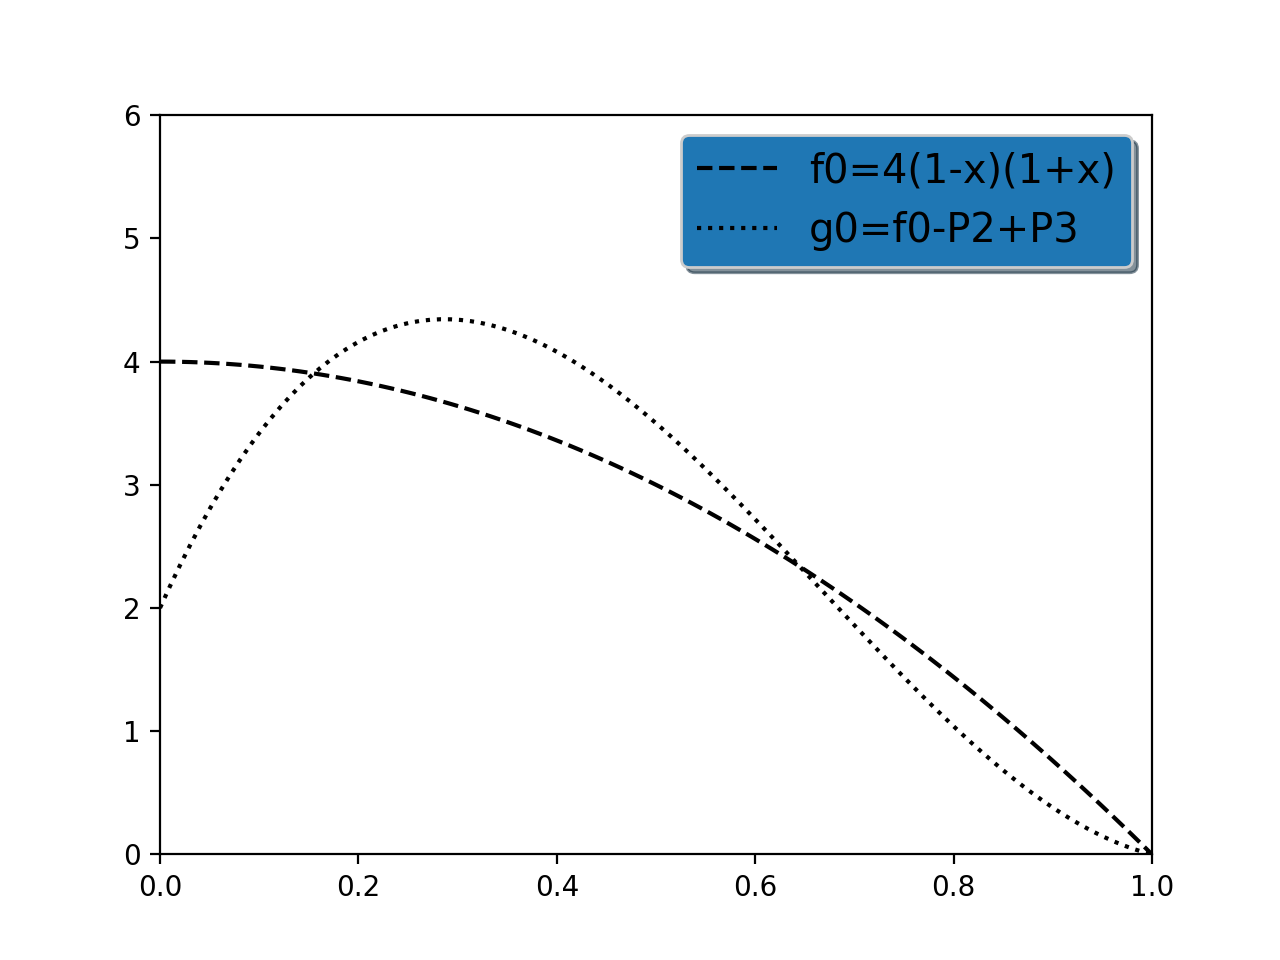
\includegraphics[width=9cm]{f0g0.png}
	

\end{preuve}
	
A écrire à partir du cours de Driss Boutat envoyé par Philippe le 18 janvier.


%%%%%%%%%%%%%%%%%%%%%%%%%%%%%%%%%%%%%%%%%%%%%%%%%%%%%%%%%%%%%%%%%%%%%%%%%%%%%%%%%%%%%%%%%%%%%%%%%%%%%%%%%%%%%%%%%%%%%%%%%%%%%%%%%
%%%%%%%%%%%%%%%%%%%%%%%%%%%%%%%%%%%%%%%%%%%%%%%%%%%%%%%%%%%%%%%%%%%%%%%%%%%%%%%%%%%%%%%%%%%%%%%%%%%%%%%%%%%%%%%%%%%%%%%%%%%%%%%%%
%%%%%%%%%%%%%%%%%%%%%%%%%%%%%%%%%%%%%%%%%%%%%%%%%%%%%%%%%%%%%%%%%%%%%%%%%%%%%%%%%%%%%%%%%%%%%%%%%%%%%%%%%%%%%%%%%%%%%%%%%%%%%%%%%
\section{Dépolymérisation - $v(t) < 0$}
%%%%%%%%%%%%%%%%%%%%%%%%%%%%%%%%%%%%%%%%%%%%%%%%%%%%%%%%%%%%%%%%%%%%%%%%%%%%%%%%%%%%%%%%%%%%%%%%%%%%%%%%%%%%%%%%%%%%%%%%%%%%%%%%%
%%%%%%%%%%%%%%%%%%%%%%%%%%%%%%%%%%%%%%%%%%%%%%%%%%%%%%%%%%%%%%%%%%%%%%%%%%%%%%%%%%%%%%%%%%%%%%%%%%%%%%%%%%%%%%%%%%%%%%%%%%%%%%%%%

Pour la suite, on considère que la vitesse $v$ est une fonction continue négative de $C^0([0,\tau],\mathbb{R}^-)$.
On s'intéresse alors à l'équation :

\begin{equation}
		\label{eq:dep}
		\begin{cases}
			\displaystyle \frac{\partial y}{\partial t}+ v(t) \frac{\partial y} {\partial x}  = 0 & (x,t) \in [0,L] \times [0, \tau] \\
             y(x,0) = y_{0} (x) \\
			 v(t)y(L,t) = 0 \\
		\end{cases}
\end{equation}



%%%%%%%%%%%%%%%%%%%%%%%%%%%%%%%%%%%%%%%%%%%%%%%%%%%%%%%%%%%%%%%%%%%%%%%%%%%%%%%%%%%%%%%%%%%%%%%%%%%%%%%%%%%%%%%%%%%%%%%%%%%%%%%%%
\subsection{Existence et unicité}
%%%%%%%%%%%%%%%%%%%%%%%%%%%%%%%%%%%%%%%%%%%%%%%%%%%%%%%%%%%%%%%%%%%%%%%%%%%%%%%%%%%%%%%%%%%%%%%%%%%%%%%%%%%%%%%%%%%%%%%%%%%%%%%%%

Nous allons reprendre la démonstration développée pour $v>0$.
La principale différence tient à la condition aux limites.
En effet, la condition n'est imposée qu'en $x=L$.

\begin{definition}
	\label{def:cauchyd}
	Soit $\tau>0$, $\mass$ et $\dep$ deux constantes de $\mathbb{R}^+$, 
	et $L>0$. 
	
	Soit $y_0 \in L^2([0,L])$.
	
	Soit $v \in C^0([0,\tau])$.
	
	Supposons que $\forall t \in[0,\tau]$, $v(t)<0$.
	
	On dit que $y \in C^0([0,\tau],L^2[0,L])$ est solution du problème de Cauchy~\eqref{eq:dep}  
	si et seulement si pour tout $t \in [0,\tau]$ et pour
	tout $\phi \in C^1([0,\tau]\times [0,L])$ telle que :
	
	\begin{equation}
		\begin{cases}
			-\int_0^t \int_0^L (\partial_t \phi +v(t)\partial \phi) y(x,t) dxdt 
			+ \int_0^L y(x,t) \phi (x,t) dx - \int_0^L y_0(x)\phi(x,0)dx =0 \\
			\phi(0,t)=0
		\end{cases}
	\end{equation}
	
\end{definition}


\begin{theoreme}
	Soit $\tau >0$, $L>0$, $y_0 \in L^2(0,L)$ et $v \in C^0([0,\tau],\mathbb{R}^-)$.
	Alors le problème de Cauchy~\eqref{eq:dep} admet une unique solution $y \in C^0([0,\tau],L^2(0,L))$ au sens de la définition~\ref{def:cauchyd}.
\end{theoreme}

\begin{preuve}
	Comme pour la polymérisation, on commence par démontrer l'unicité : 
	soit $y_1$ et $y_2$ solution du problème de Cauchy au sens de la définition~\ref{def:cauchyd}. 
	Alors on pose $y=y_1-y2$ et pour tout $t \in [0,\tau]$, $y \in C^0([0,T],L^2(0,L))$.
	Et pour toute fonction $\phi \in C^1([0,\tau] \times [0,L])$ telle que $\phi (0,\cdot)=0$ :
\begin{equation}
	\label{dem:fd}
	-\int_0^t \int_0^L (\partial_t \phi +v(t)\partial \phi) y(x,t) dxdt 
			+ \int_0^L y(x,t) \phi (x,t) dx =0
\end{equation}

	Pour $t^*$ fixé, on définit une suite de fonction $(f_n)_{n \in \mathbb(N)}$ de $C^1(\mathbb{R})$, espace fonctionnel dense dans $L^2(0,L)$, telle que :
	
\[
\begin{cases}
	f_n =0 \; \; sur \; \; (-\infty;0], & \forall n \\
	f_{n|(0,L)} \to y(\cdot,t) \in L^2(0,L) & pour \; \;  n\rightarrow \infty.
\end{cases}
\]

Pour $n \in \mathbb(N)$ on pose alors $\phi_n \in C^1([0,t]\times [0,L])$ :

\[ \phi_n(x,t) = f_n(x + \int_t^{t^*} v(s)ds), \; \forall (x,t) \in [0,t^*]\times [0,L]. \]

Par hypothèse, $v(t) \leq 0$ sur $[0, t^*]$ alors $\phi_n$ vérifie la condition $\phi (\cdot, 0)=0$.

De plus on constate que :
\[ \partial_t \phi_n = -v(t) \partial_x \phi_n \]

Alors, en posant $\phi = \phi_n$ dans~\eqref{dem:fd} il vient :

\[ \int_0^L y(x,t^*) \phi_n (x,t^*) dx =0 \]

or $\phi_n (x,t^*) = f_n(x)$ et pour $n \rightarrow \infty$ :

\[ \int_0^L y(x,t^*)^2 dx =0 \]

On a donc montré que pour tout $t^*$ de $[0,\tau]$ on a $y(\cdot, t^*) =0 $.


	
\end{preuve}


\subsection{Problème inverse}

On considère l'équation~\eqref{eq:poldep} sous la condition~\eqref{hyp:compact}, 
alors d'après la propriété~\ref{mmt},
la dépolymérisation correspond au cas où $\dep>\mass$ (ou $\tau<t^*$).

Dans ce cas, l'équation des moments~\eqref{eq:mmt} d'écrit :

\begin{equation}
\begin{cases}
\displaystyle \frac{\mathrm{d} \mu_n }{\mathrm{d}t} = v(t) n \mu_{n-1} & n>0 \\
\displaystyle \frac{\mathrm{d} \mu_0 }{\mathrm{d}t} = v(t) y_0(-\theta(t))
\end{cases}
\end{equation}

%%%%%%%%%%%%%%%%%%%%%%%%%%%%%%%%%%%%%%%
\begin{proposition}
	Soit $\tau >0$, $L>0$, $y_0 \in L^2(0,L)$ et $v \in C^0([0,\tau],\mathbb{R})$.
	
	Soit $y$ une solution classique de~\eqref{eq:dep} sur $[0,L] \times [0,\tau]$.
	
	Alors si la vitesse $v$ est strictement négative, la condition initiale peut s'écrire de façon explicite 
	en fonction de l'opérateur de moment $\Psi_n$ :
	
	\begin{equation}
		\label{mexplicit}
		y_0(x) = \frac{1}{n! v(-\theta^{-1}(x))^{n+1}} \frac{\mathrm{d}^{n+1}}{\mathrm{d}t^{n+1}} (\Psi_n(-\theta^-1(x)))
	\end{equation}
\end{proposition}
%%%%%%%%%%%%%%%%%%%%%%%%%%%%%%%%%%%%%%%

%%%%%%%%%%%%%%%%%%%%%%%%%%%%%%%%%%%%%%%
\begin{preuve}
L'équation des moments~\eqref{eq:mmt} est toujours valable, et $max(0,\theta(t))=\theta(t)$.
On en déduit donc que pour $n>0$:
\[
\begin{split}
	\frac{\mathrm{d} \Psi_n y_0 }{\mathrm{d}t} &= \frac{\mathrm{d} \mu_n }{\mathrm{d}t}\\
	                                      &= v(t) n \mu_{n-1} (t)\\
										  &= v(t)^{n} n! \mu_0(t)\\
										  &= v(t)^{n+1} n!  y_0(-\theta(t))  
\end{split}
\]
\end{preuve}
%%%%%%%%%%%%%%%%%%%%%%%%%%%%%%%%%%%%%%%

%%%%%%%%%%%%%%%%%%%%%%%%%%%%%%%%%%%%%%%%%%%%%%%%%%%%%%%%%%%%%%%%%%%%%%%%%%%%%%%%%%%%%%%%%%%%%%%%%%%%%%%%%%%%%%%%%%%%%%%%%%%%%%%%%
\subsection{Suite régularisante}
%%%%%%%%%%%%%%%%%%%%%%%%%%%%%%%%%%%%%%%%%%%%%%%%%%%%%%%%%%%%%%%%%%%%%%%%%%%%%%%%%%%%%%%%%%%%%%%%%%%%%%%%%%%%%%%%%%%%%%%%%%%%%%%%%


to be continued.


%%%%%%%%%%%%%%%%%%%%%%%%%%%%%%%%%%%%%%%%%%%%%%%%%%%%%%%%%%%%%%%%%%%%%%%%%%%%%%%%%%%%%%%%%%%%%%%%%%%%%%%%%%%%%%%%%%%%%%%%%%%%%%%%%
\subsection{Observabilité}
%%%%%%%%%%%%%%%%%%%%%%%%%%%%%%%%%%%%%%%%%%%%%%%%%%%%%%%%%%%%%%%%%%%%%%%%%%%%%%%%%%%%%%%%%%%%%%%%%%%%%%%%%%%%%%%%%%%%%%%%%%%%%%%%%


On suppose que la solution $y$ de l'équation~\eqref{eq:dep}.
Alors $y$ est à support compact inclus dans $[0,L] \times [0,\tau]$. 

On rappelle la définition des opérateurs de mesures $\Psi_n$ pour $n \geq 0$:

 \begin{equation}
	\begin{array}{ccccc}
	\Psi_n & : & L^2([0,L]) & \to & L^2([0,\tau]) \\
	 & & y_0 & \mapsto & t \to \int_0^L x^n y_0(x-\theta(t)) dx\\
	\end{array}
\end{equation}

On note les espaces vectoriels normés,
 $\mathscr{Y} = L^2 (0,L)$,
 $\mathscr{Z} = L^2 (0,\tau)$,
alors $\Psi_n$ appartient à $L^2(\mathscr{Y},\mathscr{Z})$. 

%%%%%%%%%%%%%%%%%%%%%%%%%%%%%%%%%%%%%%%%%%%%
\begin{definition}
Le système~\eqref{eq:dep} est dit observable pour la mesure $\Psi_n$ 
au temps $\tau$ s'il existe une constante $k_n$ telle que :

\begin{equation}
	\label{obs}
	\forall y_0 \in \mathscr{Y}, \quad \| \Psi_n(y_0)\|_{\mathscr{Z}}^2 \geq k_n \|y_0\|^2_{\mathscr{Y}}
\end{equation}

\end{definition}
%%%%%%%%%%%%%%%%%%%%%%%%%%%%%%%%%%%%%%%%%%%%

%%%%%%%%%%%%%%%%%%%%%%%%%%%%%%%%%%%%%%%%%%%%
\begin{proposition}
	Le système~\eqref{eq:dep} n'est pas observable pour la mesure $\Psi_n$ 
	au temps $\tau$.
\end{proposition}
%%%%%%%%%%%%%%%%%%%%%%%%%%%%%%%%%%%%%%%%%%%%

%%%%%%%%%%%%%%%%%%%%%%%%%%%%%%%%%%%%%%%%%%%%
\begin{preuve}
	On s'appuie sur la preuve de \cite{LBrivadis}
	
Pour $y$ solution de ~\eqref{eq:dep}, cette inégalité n'est pas toujours vérifiée et le système n'est pas exactement observable.

Pour la démonstration, on peut exhiber un contre exemple sous la forme d'une suite $(y_0^m)_{m \in \mathbb{N}}$ telle que :

\[
\begin{cases}
	\|y_0^m\|^2_{L^2} \underset{m\to+\infty}{\nrightarrow 0} \\
	\| \Psi_n (y_0^m)\|_{L^2}^2 \underset{m\to+\infty}{\rightarrow 0}
\end{cases}
\]
	
En effet,

\[ 
\begin{split}
	\| \Psi_n (y_0^m)\|_{L^2}^2  &= \int_0^\tau  |\int_0^l x^n y^m(x,t) dx |^2 dt \\
	                             & \leq l^{2n}  \int_0^\tau (\int_0^l y^m(x,t)dx)^2dt \\
								 & \leq l^{2n} \int_0^\tau (\int_{bt}^l y_0^m(\xi)d\xi)^2dt \\
								 & \leq l^{2n} \int_0^\tau (\int_0^l y_0^m(\xi)d\xi)^2 dt
\end{split}
\]

Il suffit donc de trouver une fonction $y_0$ telle que :

\[
\begin{cases}
	\int_0^l (y_0^m(x))^2 dx \underset{m\to+\infty}{\nrightarrow 0} \\
	\int_0^l y_0^m(\xi)d\xi \underset{m\to+\infty}{\rightarrow 0}
\end{cases}
\]

C'est le cas par exemple de la fonction :

\[
\begin{cases}
	2n^3 & 0 <x < \frac{1}{2n^2}\\
	2n - 2n^3x & \frac{1}{2n^2} <x<\frac{1}{n^2}\\
	0 & \frac{1}{n^2} <x<l
\end{cases}
\]

\end{preuve}
%%%%%%%%%%%%%%%%%%%%%%%%%%%%%%%%%

Cependant, si l'observabilité n'est pas exacte dans $L^2$, elle l'est en revanche pour l'espace de Sobolev $H^{n+1}$. 

En effet on considère maintenant lque $\Psi_n$ appartient à $H^{n+1}(\mathscr{Y},\mathscr{Z})$ avec $\mathscr{Z}=H^{n+1}(0,\tau)$. 
On munit $\mathscr{X}$ de la semi-norme pour tout $n>0$:

\begin{equation}
	\label{normH}
	\|f \|_{H^{n+1} } = \int_0^{\tau} |\frac{\mathrm{d}^{n+1}f}{\mathrm{d}t^{n+1}}|^2 dt
\end{equation}


%%%%%%%%%%%%%%%%%%%%%%%%%%%%%%%%%%%%%%%%%%%%
\begin{proposition}
	Le système~\eqref{eq:dep} est observable pour la mesure $\Psi_n$ avec $\mathscr{Z}=H^{n+1}(0,\tau)$ munie de la semi-norme~\eqref{normH} au temps $\tau$ si $ -\theta(\tau) > L$.
\end{proposition}
%%%%%%%%%%%%%%%%%%%%%%%%%%%%%%%%%%%%%%%%%%%%

\begin{preuve}
	L'équation~\eqref{mexplicit} est vérifiée :
	\[y_0(x) = \frac{1}{n! v(-\theta^{-1}(x))^{n+1}} \frac{\mathrm{d}^{n+1}}{\mathrm{d}t^{n+1}} (\Psi_ny_0(-\theta^{-1}(x)))\]
	On pose alors $ 1/k_n = n! \| v\|_{L^\infty}^{n+1}$.
	Alors:
	\[ 
		\int_0^Ly_0(x)dx \leq 1/k_n \int_0^L \frac{\mathrm{d}^{n+1}}{\mathrm{d}t^{n+1}} (\Psi_ny_0(-\theta^{-1}(x))) dx
		\]
		
	Pour $ -\theta(\tau) > L$ on peut effectuer un changement de variable et retrouver :
	
	\[ \int_0^Ly_0(x)dx \leq 1/k_n \int_0^\tau \frac{\mathrm{d}^{n+1}}{\mathrm{d}t^{n+1}} (\Psi_ny_0(t) dt \]
	
	Soit l'inégalité d'observabilite :
	
	\[\| \Psi_n(y_0)\|_{\mathscr{Z}}^2 \geq k_n \|y_0\|^2_{\mathscr{Y}}\]
	
	
	
\end{preuve}


%%%%%%%%%%%%%%%%%%%%%%%%%%%%%%%%%%%%%%%%%%%%%%%%%%%%%%%%%%%%%%%%%%%%%%%%%%%%%%%%%%%%%%%%%%%%%%%%%%%%%%%%%%%%%%%%%%%%%%%%%%%%%%%%%
%%%%%%%%%%%%%%%%%%%%%%%%%%%%%%%%%%%%%%%%%%%%%%%%%%%%%%%%%%%%%%%%%%%%%%%%%%%%%%%%%%%%%%%%%%%%%%%%%%%%%%%%%%%%%%%%%%%%%%%%%%%%%%%%%
%%%%%%%%%%%%%%%%%%%%%%%%%%%%%%%%%%%%%%%%%%%%%%%%%%%%%%%%%%%%%%%%%%%%%%%%%%%%%%%%%%%%%%%%%%%%%%%%%%%%%%%%%%%%%%%%%%%%%%%%%%%%%%%%%
\section{Analyse numérique pour la dépolymérisation}
%%%%%%%%%%%%%%%%%%%%%%%%%%%%%%%%%%%%%%%%%%%%%%%%%%%%%%%%%%%%%%%%%%%%%%%%%%%%%%%%%%%%%%%%%%%%%%%%%%%%%%%%%%%%%%%%%%%%%%%%%%%%%%%%%
%%%%%%%%%%%%%%%%%%%%%%%%%%%%%%%%%%%%%%%%%%%%%%%%%%%%%%%%%%%%%%%%%%%%%%%%%%%%%%%%%%%%%%%%%%%%%%%%%%%%%%%%%%%%%%%%%%%%%%%%%%%%%%%%%

Pour tous les développements qui suivent, on considère que $\dep>\mass$. Dans ce cas le système dépolymérise et $v(t)<0$ pour tout $t>0$.

On rappelle le système~\eqref{eq:dep} auquel on s'intéresse :

\[
\begin{cases}
		\displaystyle \frac{\partial y}{\partial t}+ v(t) \frac{\partial y} {\partial x}  = 0 & (x,t) \in [0,L] \times [0, \tau] \\
        y(x,0) = y_{0} (x) \\
	    v(t)y(L,t) = 0 \\
\end{cases}
\]

%%%%%%%%%%%%%%%%%%%%%%%%%%%%%%%%%%%%%%%%%%%%%%%%%%%%%%%%%%%%%%%%%%%%%%%%%%%%%%%%%%%%%%%%%%%%%%%%%%%%%%%%%%%%%%%%%%%%%%%%%%%%%%%%%
\subsection{Discrétisation}
%%%%%%%%%%%%%%%%%%%%%%%%%%%%%%%%%%%%%%%%%%%%%%%%%%%%%%%%%%%%%%%%%%%%%%%%%%%%%%%%%%%%%%%%%%%%%%%%%%%%%%%%%%%%%%%%%%%%%%%%%%%%%%%%%

Pour implémenter numériquement la résolution , on choisit d'approcher la solution $y$ par sa valeur sur les points d'un maillage régulier $(x_i)_{i \in [0,N_X]}$ de l'intervalle $[0,L]$ avec le pas d'espace $ delta x = x_{i+1} - x_i$ pour $i$ dans $[0,N_X-1]$. On introduit donc une approximation par morceaux de la solution :

\[ Y(t) = (y_{i=0}(t), y_{i=1}(t),...,y_{i=N_X}(t)) \; \in \mathbb{C^0}^{N_X}\]

Puisque le système ne fait que dépolymériser, c'est à dire transporter l'information vers les $x$ petits, on considère qu'il existe $L>0$ tel que quelque soit $t>0$ et $x>L$ la concentration de polymère est nulle et solution $y(x,t)=0$. On discrétise également le temps en une partition de $N_T$ points de durée $\delta t_j = t_{j+1} - t_j$ pour $j$ dans $[0,N_T-1]$. La fonction $y \in L^2$ est ainsi approximée par $\tilde{y}$ définie par :

\[ \tilde{y} (x,t) = y(x_i,t_j)=y_i^j \; \forall \; (x,t) \in \; [x_i;x_{i+1}) \times [t_j;t_{j+1)}]\]

De plus on admet la notation :

\[Y(t_j) = Y^j \; \forall j \in [0,N_T] \]

De même la vitesse peut être discrétisée et on note pour tout $j$ :

\[ v(t_j) = v_j \]

Pour résoudre ce qui suit, on ne considère pas que les $\delta t_j$ sont réguliers, contraitement à la discrétisation spatiale.

Au contraire, on considère que $\displaystyle \delta t_j = \frac{\delta x}{v_{j}} $.
Ainsi il est possible d'adopter un schéma explicite décentré gauche stable, puisqu'il s'agit d'une interpolation de la solution sur les caractéristiques, pour l'opérateur de dérivation, soit :

\[ v(t)\partial_x y = v_j \frac{y_{i+1}^j - y_{i}^j}{\delta x} \]

Soit $F_j = F(v(t_j))$ pour $J \leq 0$ l'opérateur discret tel que :

\[ \begin{cases}
F_0 = \mathbb{I} \\
Y^{j+1} = F_j Y^{j-1} 
\end{cases}\]

Pour un schéma explicite en temps, $F_j$ s'écrit :

\[
\begin{cases}
	\alpha_j = \frac{\delta t_j v_{j}}{\delta x}  \\
	 F_j  =\left( \begin{array}{cccc}
	1-\alpha_j &    \alpha_j   &  0     & 0 \\
	0      & 1-\alpha_j   & \alpha_j   & 0 \\
	0      &   0     & \ddots &  \alpha_j \\
	0      & 0       &0        & 1-\alpha_j
	 \end{array} \right)
\end{cases}
\]

On définit de plus l'opérateur $S_j$ :

\[ S_j = F_j o F_{j-1} o \cdots o F_1 o F_0 \]

Et on observe que :

\[ Y^j= S_j Y^0\]

Pour les observations, on choisit pour l'opérateur intégrale une méthode des trapèzes :

\[ z(t_j) = z_j = CY^j\]

Avec :
\[
C =  \left( \begin{array}{cc}
	\frac{\delta x}{2} x_0       &  \frac{\delta x}{2}x_0^2   \\
	\delta x x_1       &  \delta xh x_1^2   \\
	\vdots      & \vdots     \\
	\delta x x_{NX-2}  & \delta xx_{NX-2}^2\\
    \frac{\delta x}{2} x_{NX-1}  & \frac{\delta x}{2} x_{NX-1}^2
	 \end{array} \right)
\]


%%%%%%%%%%%%%%%%%%%%%%%%%%%%%%%%%%%%%%%%%%%%%%%%%%%%%%%%%%%%%%%%%%%%%%%%%%%%%%%%%%%%%%%%%%%%%%%%%%%%%%%%%%%%%%%%%%%%%%%%%%%%%%%%%
\subsection{Filtre de Kalman}
%%%%%%%%%%%%%%%%%%%%%%%%%%%%%%%%%%%%%%%%%%%%%%%%%%%%%%%%%%%%%%%%%%%%%%%%%%%%%%%%%%%%%%%%%%%%%%%%%%%%%%%%%%%%%%%%%%%%%%%%%%%%%%%%%

Grâce aux notations introduites ci-dessus, on peut définir le critère discret $J$ que l'on souhaite discrétiser :
\[
\begin{split}
    J(\zeta,N_T) &= \frac{1}{2}\alpha \parallel \zeta \parallel _{N_{\diamond},\mathscr{Y}}^2 + \frac{1}{2}\gamma \sum_{j=0}^{NTT} \delta t_j \parallel z_j - CS_j(y_{\diamond}+\zeta) \parallel_{M_j,\mathscr{Z}}^2 \\
	                 &= \frac{1}{2}\alpha \zeta ^T N_{\diamond} \zeta + \frac{1}{2}\gamma \sum_{j=0}^{NTT} \delta t_j (z_j - CS_j(y_{\diamond}+\zeta)^T M_j (z - CS_j(y_{\diamond}+\zeta))\\
					 &=  \frac{1}{2}\alpha \zeta ^T N_{\diamond} \zeta + \frac{1}{2}\gamma \delta t \sum_{j=0}^{NTT} (C S_j\zeta)^T M_jCS_j\zeta
			            -2(z_j-CS_jy_{\diamond})^TM_jCS_j \zeta + cste\\
					 &= 1/2 \zeta^T A_{N_T} \zeta - b_{N_T}^T\zeta
\end{split}
\]

Le minimiseur de $J$ noté $\hat{\zeta}$ vérifie la propriété :

\[
\mathrm{d}_{\zeta} J{\hat{\zeta},N_T} = 0
\]

Soit :

\[ \hat{\zeta}= A_{N_T}^{-1} b_{N_T} \]

Dans un premier temps, on construit la suite $\zeta_{|n}$ qui vérifie les relations suivantes :

\begin{equation}
	\begin{cases}
		\displaystyle A_n = (\alpha N_{\diamond} + \gamma  \sum_{j=0}^{n}\delta t_j S_j^TC^TM_jCS_j)\\
		b_n = \gamma \sum_{j=0}^{n} \delta t_j  S_j^T C^T M_j(z(t_j)-CG^jy_{\diamond}) \\
		\hat{\zeta}_{|n} = argmin J(\cdot,n) \\
		A_n \hat{\zeta}_{|n} = b_n
	\end{cases}
\end{equation}


Soit la matrice de norme $\tilde{M}_n= \gamma \delta t_n M_n$.


On utilise le lemme d'inversion matricielle pour trouver une relation de récurrence entre $A_n$ et $A_{n-1}$ et il vient :

\[\zeta_{|n} = \zeta_{|n-1} + A_{n}^{-1} \S_n^T C^T \tilde{M}_n (z_n- C S_n (y_{\diamond} + \zeta_{|n-1}) ) \]

Dans un deuxième temps, on construit la suite donnée par le filtre de Kalman $y_{n|n}$ telle que :

\[
\begin{cases}
	y_{0|n} = y_{\diamond} + \zeta_{|n} \\
	y_{n|n} = S_n y_{0|n} 
\end{cases}
\]

La relation de récurrence entre $y_{n|n}$ et $y_{n-1|n-1}$ est donnée par :

\[
\begin{split}
y_{n|n} &= S_n (y_{\diamond} + \zeta_{|n}) \\
        &= S_n (y_{\diamond} + \zeta_{|n-1}) + S_n A_{n}^{-1}S_n^T C^T \tilde{M}_n (z_n-C S_n y_{0|n-1}) \\
		&= F_n y_{n-1|n-1} + (S_nA_{n}^{-1} S_n^TC^T \tilde{M}_n (z_n -CF_n( S_{n-1} y_{0|n-1})) \\
		&= F_n y_{n-1|n-1} + P_n C^T \tilde{M}_n (z(t_n)-CF_ny_{n-1|n-1})		
\end{split}
\]


De part cette expression on peut reconstruire en deux étapes la dynamique de l'estimateur de Kalman discret $\hat{y}_n = y_{n|n}$ : 

\[
\begin{cases}
		\text{Initialisation :}\\
		P_0^- = P_{\diamond} = \mathbb{I} \\
		\hat{y}_0^- = y_{\diamond} \\
		\text{Correction :}\\
		K_n = P_n^- C^T (\tilde{M}_n^{-1} + C^TP_n^-C)^-1 \\
		P_n^+ = (\mathbb{I} - K_nC)P_n^-(\mathbb{I}-K_nC)^T + K_n \tilde{M}_n^{-1} K_n^T\\
		\hat{y}_n^+ = \hat{y}_n^- + P_n^+C^T \tilde{M}_n ( z_n - C \hat{y}_n^-)\\
		\text{Prediction :}\\
		P_{n+1}^- = F_n P_n^+ F_n^T
		\hat{y}_{n+1}^- = F_n \hat{y}_n^+
	\end{cases}
\]
   
%%%%%%%%%%%%%%%%%%%%%%%%%%%%%%%%%
%%%%%%%%%%%%%%%%%%%%%%%%%%%%%%%%%
%%%%%%%%%%%%%%%%%%%%%%%%%%%%%%%%%

\section{Conclusion}
%%%%%%%%%%%%%%%%%%%%%%%%%%%%%%%%%

To be continued.

%%%%%%%%%%%%%%%%%%%%%%%%%%%%%%%%%%%%%%%%%%%%%%%%%%%%%%%%%%%%%%%%%%%%%%%%%%% REFERENCES

\medskip

\bibliographystyle{unsrt}%Used BibTeX style is unsrt
\bibliography{20190118biblio}
	
\end{document}
